\documentclass[class=article,border=5pt,tikz]{standalone}
\usetikzlibrary{arrows.meta}

\begin{document}

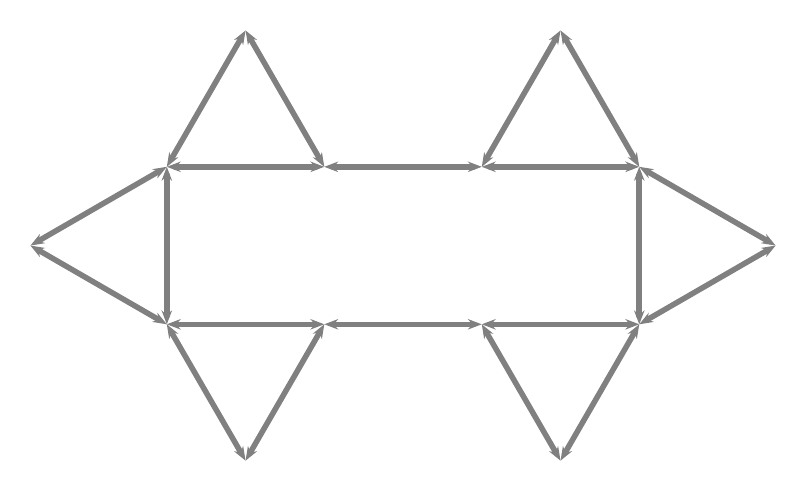
\begin{tikzpicture}[very thick, line width=2pt, line cap=round, line join=round, >={Stealth[length=5pt]}, color=gray, scale=2]
\draw [<->] (0,0) -- (1,0); 
\draw [<->] (1,0) -- (2,0); 
\draw [<->] (2,0) -- (3,0); 
\draw [<->] (3,0) -- (3,1); 
\draw [<->] (3,1) -- (2,1); 
\draw [<->] (2,1) -- (1,1);
\draw [<->] (1,1) -- (0,1);
\draw [<->] (0,1) -- (0,0);
\draw [<->] (0,1) -- (0.5,1.866);
\draw [<->] (0.5,1.866) -- (1,1);
\draw [<->] (2,1) -- (2.5,1.866);
\draw [<->] (2.5,1.866) -- (3,1);
\draw [<->] (0,0) -- (0.5,-0.866);
\draw [<->] (0.5,-0.866) -- (1,0);
\draw [<->] (2,0) -- (2.5,-0.866);
\draw [<->] (2.5,-0.866) -- (3,0);
\draw [<->] (0,0) -- (-0.866,0.5);
\draw [<->] (-0.866,0.5) -- (0,1);
\draw [<->] (3,0) -- (3.866,0.5);
\draw [<->] (3.866,0.5) -- (3,1);
\end{tikzpicture}


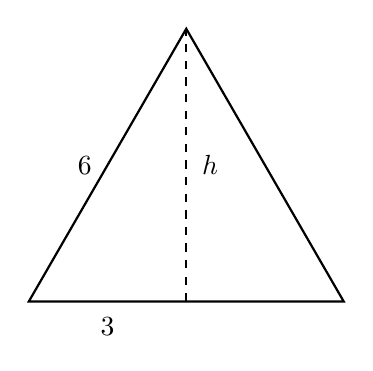
\begin{tikzpicture}[thick, sharp corners, inner sep=1mm, outer sep =1mm, scale=4]
\draw (0,0) -- (0.5,0) node[midway,below]{$3$} -- (1,0) -- (0.5, 0.866) -- cycle node[midway,left]{$6$}; 
\draw[dashed] (0.5,0) -- (0.5,0.866) node[midway,right]{$h$};
\end{tikzpicture}
\end{document}
